\documentclass{article}
\usepackage{tikz}
\usetikzlibrary{decorations.markings}
\pagestyle{empty}
\begin{document}
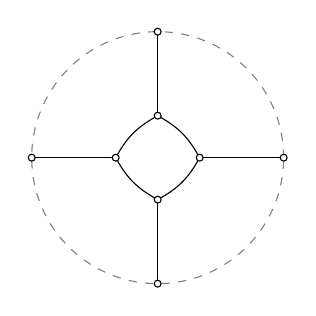
\begin{tikzpicture}
[scale=1.6,every node/.style={draw, circle, fill=white, inner sep=0pt, outer sep=0pt, minimum size=2.5pt},
->-/.style={decoration={markings, mark=at position .5 with{\arrow{>}}}, postaction={decorate}},
-<-/.style={decoration={markings, mark=at position .5 with{\arrow{<}}}, postaction={decorate}}]
\draw[gray, dashed] (0,0) circle (1.0);
 \node (5) at (0.0,1.0) {};
\node (6) at (-1.0,0.0) {};
\node (7) at (-0.0,-1.0) {};
\node (8) at (1.0,-0.0) {};
\node (1) at (0.3333,-0.0) {};
\node (2) at (-0.0,0.3333) {};
\node (3) at (-0.0,-0.3333) {};
\node (4) at (-0.3333,-0.0) {};
\draw[out=180.0, in=0.0] (8) to (1);
\draw[out=90.0, in=270.0] (7) to (3);
\draw[out=-0.0, in=180.0] (6) to (4);
\draw[out=-90.0, in=90.0] (5) to (2);
\draw[out=120.0, in=330.0] (1) to (2);
\draw[out=240.0, in=390.0] (1) to (3);
\draw[out=510.0, in=300.0] (3) to (4);
\draw[out=210.0, in=420.0] (2) to (4);
\end{tikzpicture}
\end{document}